\subsection{A physically actuated S-shaped endpoint path}
\label{sec:s-path}
The moving clamped base permitted by the distributed formulation supplies
an axial feed coordinate $b(t)$, while the same single transverse magnetic
field bends the catheter. In the Cartesian small-slope model,
the centreline is
\begin{equation}
 \begin{aligned}
 r(s,t)&=\bigl(b(t)+s,w(s,t)\bigr),\\
 r_{\rm tip}(t)&=\bigl(b(t)+L,w(L,t)\bigr).
 \end{aligned}
 \label{eq:s-path-geometry}
\end{equation}
The axial feed and magnetic bending together prescribe the endpoint
history. The material length remains
$80$ mm throughout; advancing a varying length through a guide is a
different boundary-value problem.

The base starts at rest. Over the first second its speed is
$\dot b=v_b(10\xi^3-15\xi^4+6\xi^5)$, where $\xi=t/(1\,\mathrm{s})$
and $v_b=4\,\mathrm{mm\,s^{-1}}$; afterwards $\dot b=v_b$.
The transverse request is zero until $2$ s. During the subsequent
$12$ s stroke, put $\sigma=(t-2\,\mathrm{s})/(12\,\mathrm{s})$ and prescribe
\begin{equation}
 y_r(t)=\frac{8A}{3\sqrt3}
       \left(\frac12\sin 2\pi\sigma-\frac14\sin4\pi\sigma\right),
 \quad A=1.5\,\mathrm{mm}.
 \label{eq:s-path-reference}
\end{equation}
Outside this interval $y_r=0$. Its position, velocity and acceleration
join continuously to zero, and its two lateral extrema are $\pm A$.
The resulting S-shaped endpoint stroke advances $48$ mm axially.
The base acceleration is at most $7.5\,\mathrm{mm\,s^{-2}}$ and ends
before any bending command is applied. Consequently the beam is exactly
straight during axial acceleration and the base has zero acceleration
throughout the bending stroke. There is no axial fluid load, guide friction,
or imposed axial prestress in this test.

\paragraph{Base work and clearance.}
Let $m_b=\rho A_cL$ denote the rod mass, with $A_c$ its cross-sectional area.
Orthogonality of the axial and transverse Cartesian velocities gives
\begin{equation}
 E_{\rm total}=E_\perp+\frac12m_b\dot b^2,
 \qquad P_b=F_b\dot b=m_b\ddot b\dot b.
 \label{eq:s-path-base-energy}
\end{equation}
Here $E_\perp$ is the same transverse kinetic, bending and static-field
energy used in the clearance theorem. The chosen timing also avoids
transverse geometric-stiffness effects from an accelerating bent beam:
the axial inertial load acts only while $w=0$. During bending, axial
translation is force-free in the stated model. Thus
\begin{equation}
 \dot E_{\rm total}
 =\mu B_y\cos\vartheta\,\dot\vartheta
  -\alpha\dot q^{\mathsf T}M\dot q+P_b.
 \label{eq:s-path-total-power}
\end{equation}
The base work is $W_b=m_b\dot b^2/2$ and is accounted for separately
from the magnetic input budget.
The straight, open-ended corridor is invariant under axial translation.
Its lateral noncollision proof therefore applies to $E_\perp$ and the
actual magnetic port, while the separate base-energy balance is retained.
For the same $4$ mm net clearance and $0.95E_c$ transverse work cap,
the continuous-time centreline bound remains $3.898718$ mm.
This statement would require additional work and geometry terms for
curved walls, axial contact, variable insertion length or axial drag.

\paragraph{Learned control and comparisons.}
The conservative readout is the integral fit to full-FE COMSOL
position--velocity data in Section~\ref{sec:comsol-identification}.
It has cosine multiplier $1.0223248822$ and includes all fitted quartic
terms; its invariant torus is certified independently. The conservative
coefficients and the nonnegative drag readout are held fixed throughout
this experiment. The controller evaluates its drift and
magnetic input gain from the complete learned gradient and Hessian,
as in the preceding tracking construction. For this experiment the
feedback error uses the actual full-beam tip position and velocity;
the first two modal projections supply the learned drift and gain.
The request is clipped to $|B_y|\leq20$ mT and passed through the
same physical input-work governor. Every plant run integrates all
$64$ FE degrees of freedom. The imposed base motion has the same
force and speed budget in every comparison.

\begin{table*}[t]
\centering\small
\caption{S-path tracking on the full FE plant. RMS errors use the 12 s
stroke; maxima use the full 16 s simulation. All baselines share the
same trajectory, physical input and field bound.}
\label{tab:s-path}
\begin{tabular}{lrr}
\hline
Controller & RMS ($\mu$m) & Max. ($\mu$m)\\
\hline
CHNN, measured tip feedback & 6.419 & 12.907\\
Quadratic model, measured tip feedback & 6.207 & 12.476\\
Known-physics static inverse feedforward & 4.124 & 8.005\\
CHNN, modal-output feedback & 25.308 & 41.544\\
\hline
\end{tabular}
\end{table*}

The known-physics static inverse has the smallest tracking error in
Table~\ref{tab:s-path} for this slow, weakly nonlinear nominal trajectory.
The learned controller also follows the S-shaped endpoint path, with
accuracy depending on the measured output: full-tip feedback reduces
the CHNN error relative to its two-mode reconstruction while using
the same fitted energy and physical input.

The learned controller uses a peak field of $12.9177$ mT and a sampled
peak field slew of $10.4268\,\mathrm{mT\,s^{-1}}$. Its largest
centreline displacement is $1.48892$ mm, leaving $2.51108$ mm of
net lateral clearance at the saved times; the largest slope is
$0.03718$ rad. The recorded work-based energy estimate peaks at $4.84997$ nJ,
below the $22.66365$ nJ cap, and neither field saturation nor governor
intervention occurs. The base's maximum kinetic energy is $0.796205$ nJ,
its peak ideal inertial force is $0.746442\,\mu$N, and its peak power
is $1.90256$ nW. Numerical total-energy balance includes this base work
and has maximum residual $2.44\times10^{-18}$ J.
Tightening integration tolerances by a factor of ten and halving the
maximum step changes the tip by at most $3.14\times10^{-12}$ m and
the commanded field by at most $1.47\times10^{-10}$ T at saved times.

\paragraph{Independent COMSOL field replay.}
An additional COMSOL solve integrates the same full beam for $16$ s
using the saved learned-controller field, with piecewise-cubic field
interpolation, generalized-alpha integration, relative tolerance
$10^{-8}$ and maximum step $0.002$ s. The prescribed field is the
controller output from the preceding simulation. Its tip differs from the
Python result by $1.312\times10^{-10}$ m RMS and at most
$4.038\times10^{-10}$ m, and its S-stroke tracking RMSE is
$6.419\,\mu$m. COMSOL independently integrates the mechanical
response to this prescribed command; the controller is not recomputed
online in this replay. Axial translation is reconstructed using the same analytic
base protocol. Power balance reconstructed by trapezoidal integration
of the $0.004$ s output samples has a $1.244\times10^{-14}$ J residual;
this diagnostic is distinguished from the much tighter internal Python
work-state integration and is not used as a rigorous solver-error bound.

\begin{figure*}[t]
\centering
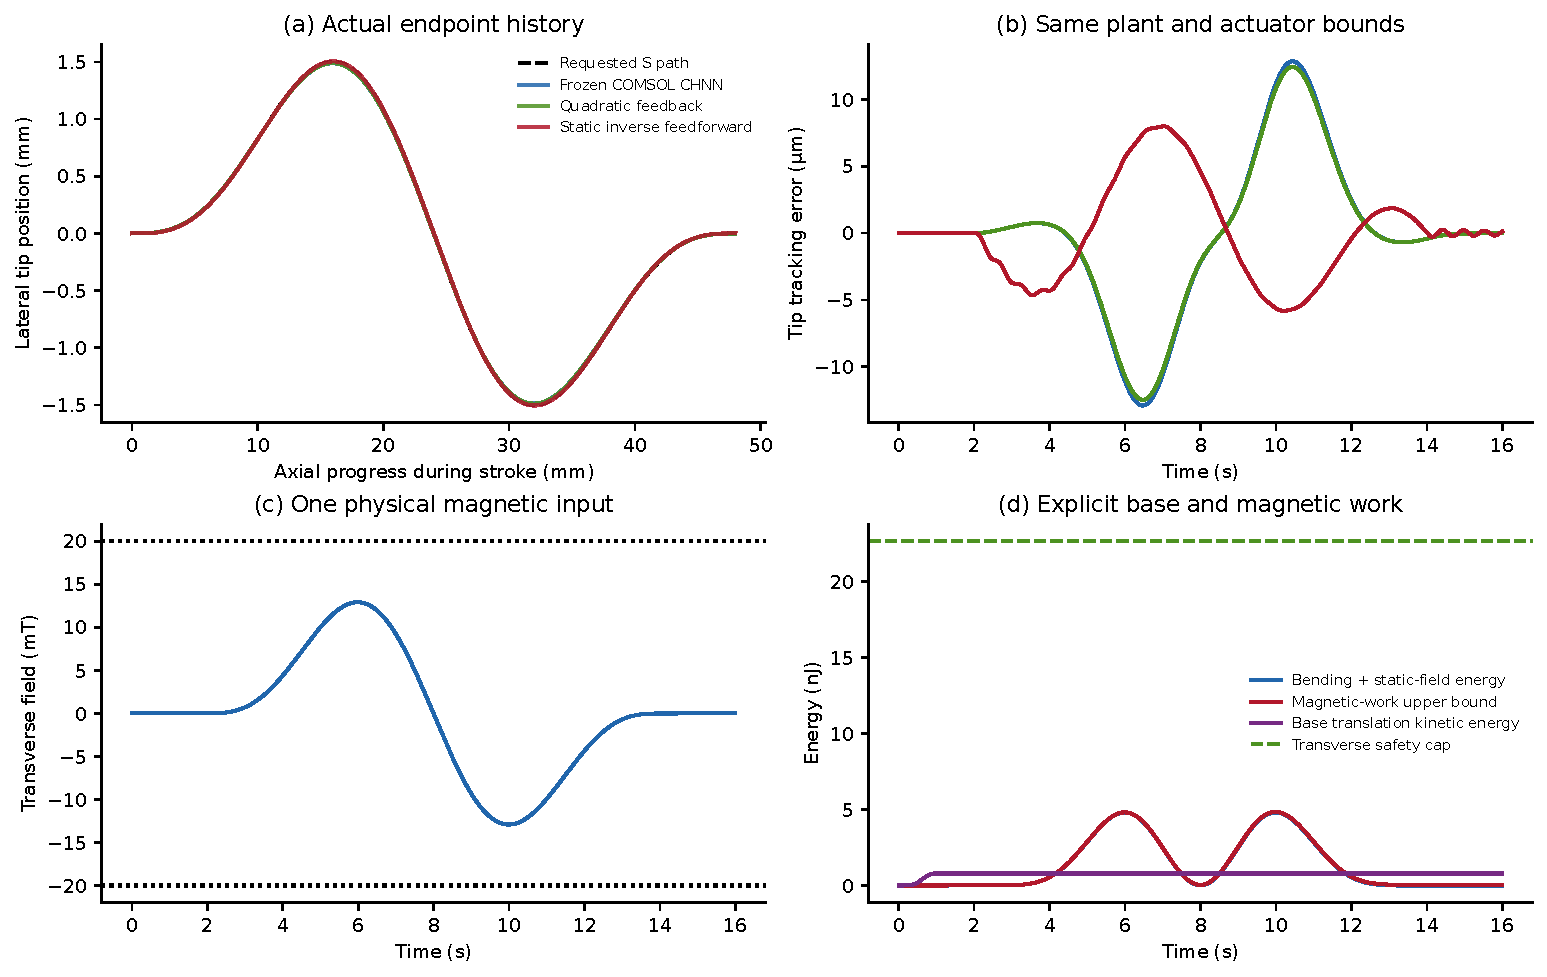
\includegraphics[width=\textwidth]{figures/fig_s_path_tracking.pdf}
\caption{A realized S-shaped endpoint path generated by axial base feed
and one transverse magnetic input. The controller uses the fitted
COMSOL-trained CHNN on the full FE plant. Axial translation work is
explicitly included in the energy balance. The matched controls reveal
that known-physics static inverse feedforward is more accurate on this
particular slow nominal path.}
\label{fig:s-path}
\end{figure*}
